\documentclass[aspectratio=169]{beamer}
\usetheme[progressbar=frametitle, numbering=fraction]{metropolis}
 % Modern, minimal theme
\setbeamertemplate{footline}{
  \leavevmode%
  \hbox{%
  \begin{beamercolorbox}[wd=.95\paperwidth,ht=2.5ex,dp=1ex,leftskip=1em]{author in head/foot}%
    \usebeamerfont{author in head/foot}\insertshortauthor\hspace{1em}-- \insertshortinstitute
  \end{beamercolorbox}%
  \begin{beamercolorbox}[wd=.3\paperwidth,ht=2.5ex,dp=1ex,rightskip=1em]{date in head/foot}%
    \usebeamerfont{date in head/foot}\insertframenumber{} / \inserttotalframenumber
  \end{beamercolorbox}}%
}

\usepackage{graphicx}   % Images
\usepackage{minted}
\usepackage{booktabs}   % Tables
\usepackage{amsmath}    % Math support
\usepackage{minted} 
\usepackage{caption}
% Code blocks (use -shell-escape to compile)
\usepackage{tikz}       % Diagrams (optional)

% Title Info
\title{I/O Performance trade-offs among persistent layouts of RNTuple }
\subtitle{}
\author{S M Shovan}
\institute{Fermilab National Laboratory}
\date{\today}

\begin{document}

% Title Slide
\maketitle

% Outline
\begin{frame}{Outline}
\tableofcontents
\end{frame}

\begin{frame}{Context}
  \begin{itemize}
    \item ROOT is a C++ framework developed at CERN for high-energy physics (HEP) data analysis and storage.
    \item Traditional storage uses TTree: columnar format for event-based data, but limited in scalability for exascale datasets.
    \item RNTuple is ROOT's next-generation columnar storage, offering improved compression, I/O performance, and flexibility.
    \item This project benchmarks RNTuple I/O configurations using simulated hit and wire data from particle detectors.
    \item Key data structures: Hits (particle interactions) and Wires (detector signals with ROIs).
  \end{itemize}
\end{frame}

\begin{frame}{Motivation}
  \begin{itemize}
    \item HEP experiments generate petabytes of data; efficient I/O is critical for analysis workflows.
    \item RNTuple aims to outperform TTree in read/write speeds, file sizes, and multi-threaded access.
    \item Explore persistent layouts (e.g., vector vs. individual, split, spills) to optimize for real-world detector data patterns.
    \item Enable scalable parallel processing, reducing time-to-insight in large-scale simulations and experiments.
  \end{itemize}
\end{frame}

\begin{frame}{Problem Statement}
  \begin{itemize}
    \item How do different RNTuple layouts affect I/O performance for hierarchical data like hits and wires?
    \item Evaluate trade-offs: file size, write times, cold/warm read times, and scaling with threads.
    \item Challenges: Balancing granularity for queries vs. overhead in entry counts; ensuring thread-safety in generation and I/O.
    \item Goal: Identify optimal configurations for HEP workloads, using benchmarks on generated datasets (e.g., 1M hits, 100K wires).
  \end{itemize}
\end{frame}

\begin{frame}{Objectives}
  \begin{itemize}
    \item Benchmark RNTuple's I/O performance across diverse persistent layouts (vector, individual, split, spills) using simulated HEP data.
    \item Measure key metrics: write times, cold/warm read times, file sizes, and multi-threaded scaling.
    \item Analyze trade-offs between granularity, compression, and parallel efficiency for hierarchical datasets like hits and wires.
    \item Identify optimal configurations for high-throughput HEP workflows, enhancing ROOT's data handling capabilities.
    \item Provide actionable insights to guide RNTuple adoption in large-scale experiments.
  \end{itemize}
\end{frame}

% -------- Section: Persistent Layouts --------
\section{Persistent Layouts}
\begin{frame}{Data Layouts: AOS vs. SOA}
  \begin{columns}
    \column{0.5\textwidth}
    \textbf{Array of Structures (AOS)} \\
    \small Stores complete objects in an array. Good for row-wise access.
    \vspace{0.5em}\\
    \texttt{struct HitIndividual \{ long long EventID; unsigned int fChannel; float fPeakTime; \};} \\
    \texttt{// Array: [Hit1, Hit2, ...]}
    \vspace{0.5em}\\
    \textbf{Example}: HitIndividual, WireIndividual (per-item entries).

    \column{0.5\textwidth}
    \textbf{Structure of Arrays (SOA)} \\
    \small Separate arrays per field. Optimized for columnar I/O.
    \vspace{0.5em}\\
    \texttt{struct HitVector \{ vector<unsigned int> fChannel; vector<float> fPeakTime; \};} \\
    \texttt{// Columns: fChannel[ ], fPeakTime[ ], ...}
    \vspace{0.5em}\\
    \textbf{Example}: HitVector, WireVector (per-event vectors).
  \end{columns}
  \vspace{1em}
  \textbf{Project Use}: AOS for granular queries; SOA for batch efficiency in RNTuple storage.
\end{frame}

\begin{frame}{ROI Flattening vs. Custom Dictionary}
  \begin{columns}
    \column{0.5\textwidth}
    \textbf{ROI Flattening (Non-Dictionary)}
    \small Flattens hierarchical ROI data into vectors for efficient storage without custom classes.
    \vspace{0.5em}
    \texttt{struct WireVector \{} \\
    \texttt{    vector<unsigned int> fSignalROI\_nROIs;} \\
    \texttt{    vector<size\_t> fSignalROI\_offsets;} \\
    \texttt{    vector<float> fSignalROI\_data;} \\
    \texttt{\};} \\
    \vspace{0.5em}
    \textbf{Example}: Used in non-dictionary experiments for raw vector-based I/O.

    \column{0.5\textwidth}
    \textbf{Custom Dictionary (ROOT Classes)}
    \small Uses structured classes with ClassDef for ROOT's dictionary system, enabling object-oriented I/O.
    \vspace{0.5em}
    \texttt{struct RegionOfInterest \{} \\
    \texttt{    size\_t offset;} \\
    \texttt{    vector<float> data;} \\
    \texttt{    ClassDef(RegionOfInterest, 3)} \\
    \texttt{\};} \\
    \vspace{0.5em}
    \textbf{Example}: Used in dictionary experiments for type-safe, hierarchical data handling.
  \end{columns}
  \vspace{1em}
  \textbf{Project Use}: Flattening optimizes for speed; dictionaries provide better data integrity and queryability.
\end{frame}

\begin{frame}{Layout Strategies}
  % Add your content here
\end{frame}

\begin{frame}{Memory/Data Considerations}
  % Add your content here
\end{frame}

\begin{frame}{Memory/Data Considerations}
% Add your content here
\end{frame}

\section{Parallel Optimizations}
\begin{frame}{Write Optimization: Multi-Threaded Chunking}
  \begin{columns}
    \column{0.5\textwidth}
    \textbf{Parallel Chunking}
    \small Divide events into thread-specific ranges for concurrent generation and filling.
    \vspace{0.5em}\\
    \texttt{std::vector<unsigned int> seeds = generateSeeds(nThreads);} \\
    \texttt{for (int th = 0; th < nThreads; ++th) \{}
    \texttt{    int first = th * chunkSize;} \\
    \texttt{    int last = std::min(first + chunkSize, totalEvents);} \\
    \texttt{    futures.emplace\_back(std::async(} \\
    \texttt{        std::launch::async, thinWorkFunc, first, last, seeds[th], th} 
    \texttt{    ));} 
    \texttt{\}} 
    \vspace{0.5em}\\
    \textbf{Example}: From \texttt{executeInParallel} in writers.

    \column{0.5\textwidth}
    \textbf{Synchronized Filling}
    \small Use mutex to safely flush clusters after filling.
    \vspace{0.5em}\\
    \texttt{\{ std::lock\_guard<std::mutex> lock(mutex); } \\
    \texttt{    hitContext.FlushCluster(); \}} \\
    \vspace{0.5em}\\
    \textbf{Project Use}: Scales writes with cores for large datasets.
  \end{columns}
\end{frame}

\begin{frame}{Read Optimization: Cluster-Aware Splitting}
  \begin{columns}
    \column{0.5\textwidth}
    \textbf{Cluster Splitting}
    \small Split read ranges by cluster boundaries to avoid duplicates.
    \vspace{0.5em}\\
    \texttt{auto clusters = split\_range\_by\_clusters(*reader, nChunks);} \\
    \texttt{for (auto\& chunk : clusters) \{} \\
    \texttt{    futures.push\_back(std::async(} \\
    \texttt{        \&processChunk, chunk.first, chunk.second} \\
    \texttt{    ));} \\
    \texttt{\}} \\
    \vspace{0.5em}\\
    \textbf{Example}: From read functions in \texttt{HitWireReaders.cpp}.

    \column{0.5\textwidth}
    \textbf{Benefits}
    \small Prevents redundant reads, optimizes multi-threaded access.
    \vspace{0.5em}\\
    \texttt{std::vector<std::pair<size\_t, size\_t>>} \\
    \texttt{split\_range\_by\_clusters(ROOT::RNTupleReader\& reader, int nChunks)} \\
    \vspace{0.5em}\\
    \textbf{Project Use}: Enhances warm read efficiency.
  \end{columns}
\end{frame}


% -------- Section: Challenges --------
\begin{frame}{Parallel Write Challenge: File Corruption Solution}
  \begin{columns}
    \column{0.5\textwidth}
    \textbf{Problem: Concurrent Flushes}
    \small Unsynchronized cluster flushes cause file corruption in multi-threaded writes.
    \vspace{0.5em}
    \textbf{Example Issue}: Threads overwriting shared file regions.

    \column{0.5\textwidth}
    \textbf{Solution: Mutex Synchronization}
    \small Lock during flushes to serialize access per cluster.
    \vspace{0.5em}
    \texttt{for (int idx = first; idx < last; ++idx) \{} \\
    \texttt{  // Generate data for hits/wires} \\
    \texttt{  if (hitStatus.ShouldFlushCluster()) \{} \\
    \texttt{    hitContext.FlushColumns();} \\
    \texttt{    \{ std::lock\_guard<std::mutex> lock(mutex); \} } \\
    \texttt{    hitContext.FlushCluster(); \} } \\
    \texttt{  \} } \\
    \texttt{\}} \\
    \vspace{0.5em}
    \textbf{Project Use}: Ensures thread-safe parallel writes without corruption.
  \end{columns}
\end{frame}

\begin{frame}{Limitations}
% Add your content here
\end{frame}

% -------- Section: Results --------
% -------- Section: Results --------
\section{Results}

\begin{frame}{Evaluation Metrics}
% Add your content here
\end{frame}

\begin{frame}{Performance Analysis}
% Add your content here
\end{frame}

\begin{frame}{Experiment 1}
\centering
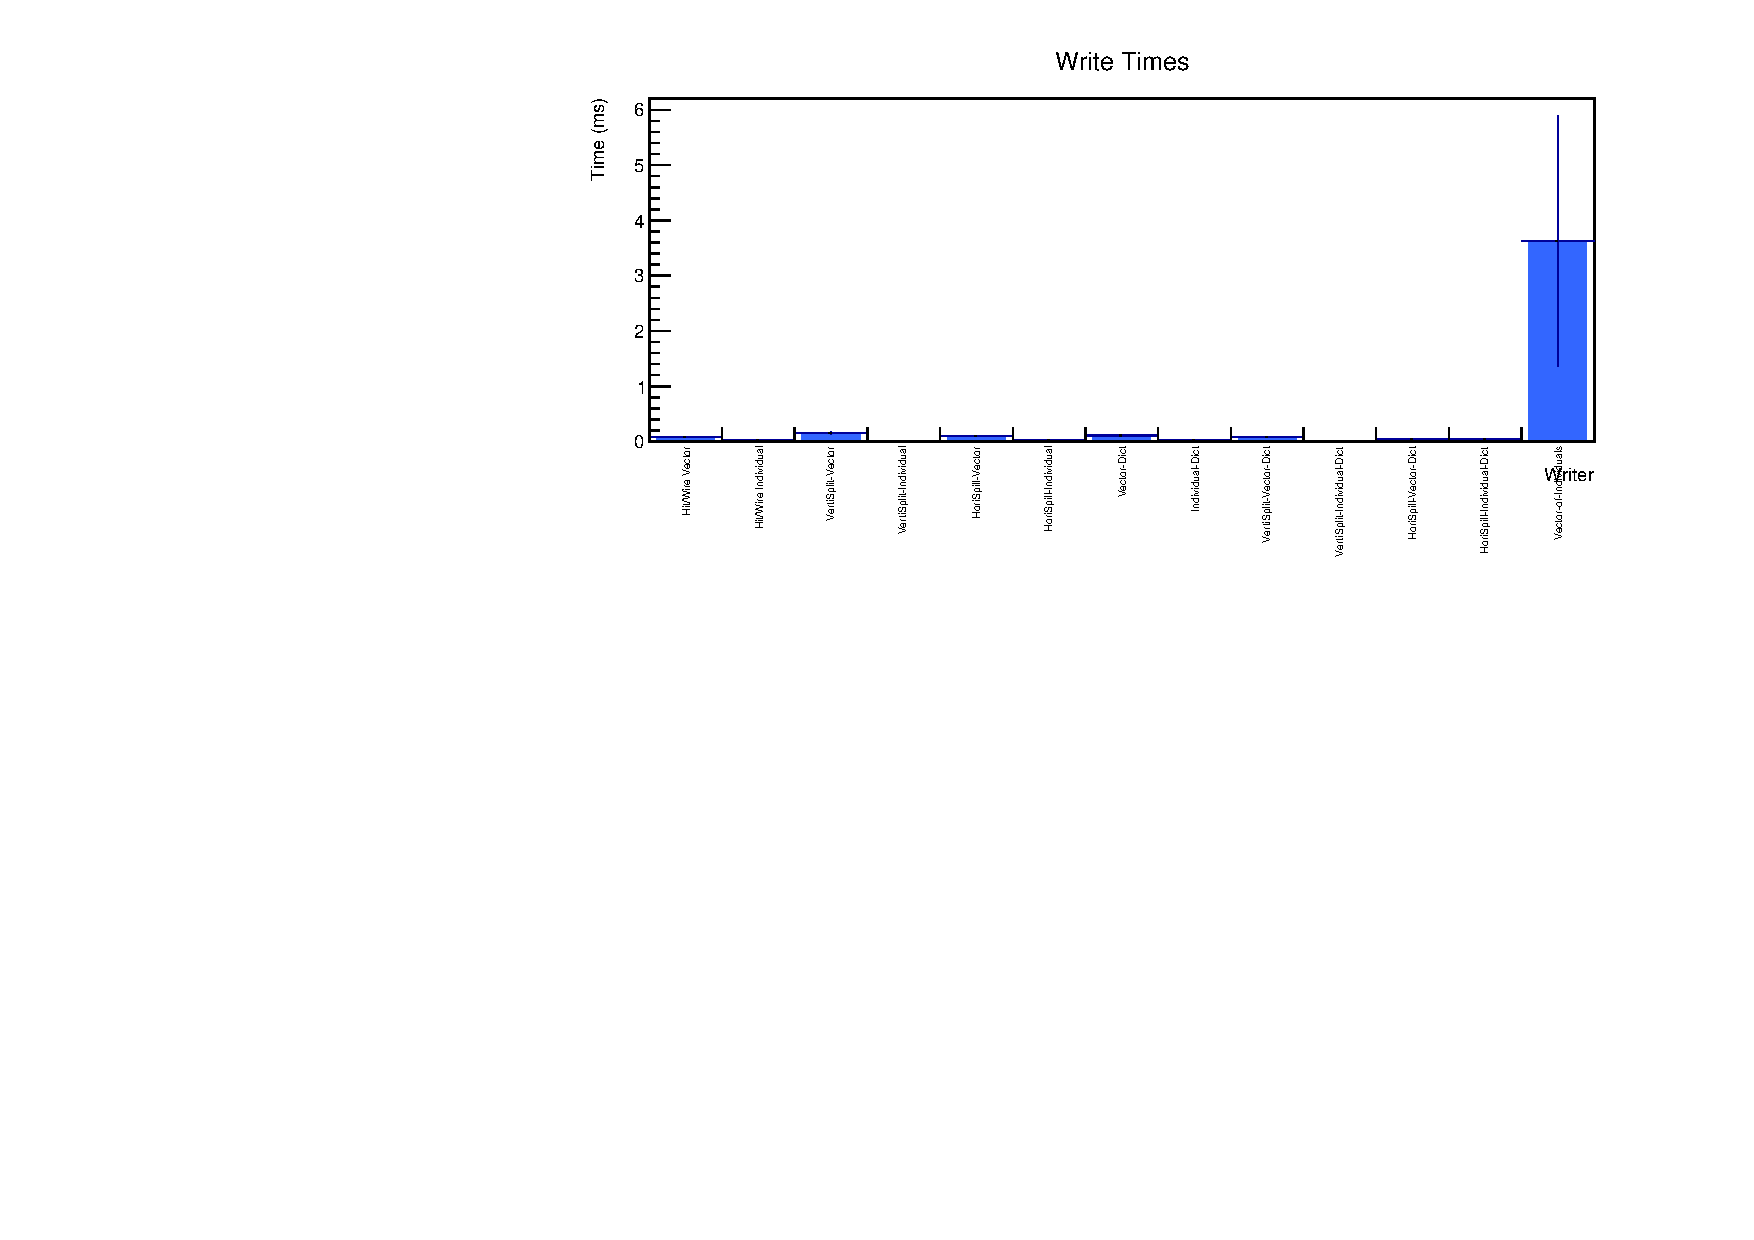
\includegraphics[width=0.9\linewidth]{../experiments/write_times.pdf}
\captionof{figure}{Experiment 1: Description goes here.}
\end{frame}

\begin{frame}{Experiment 2}
\centering
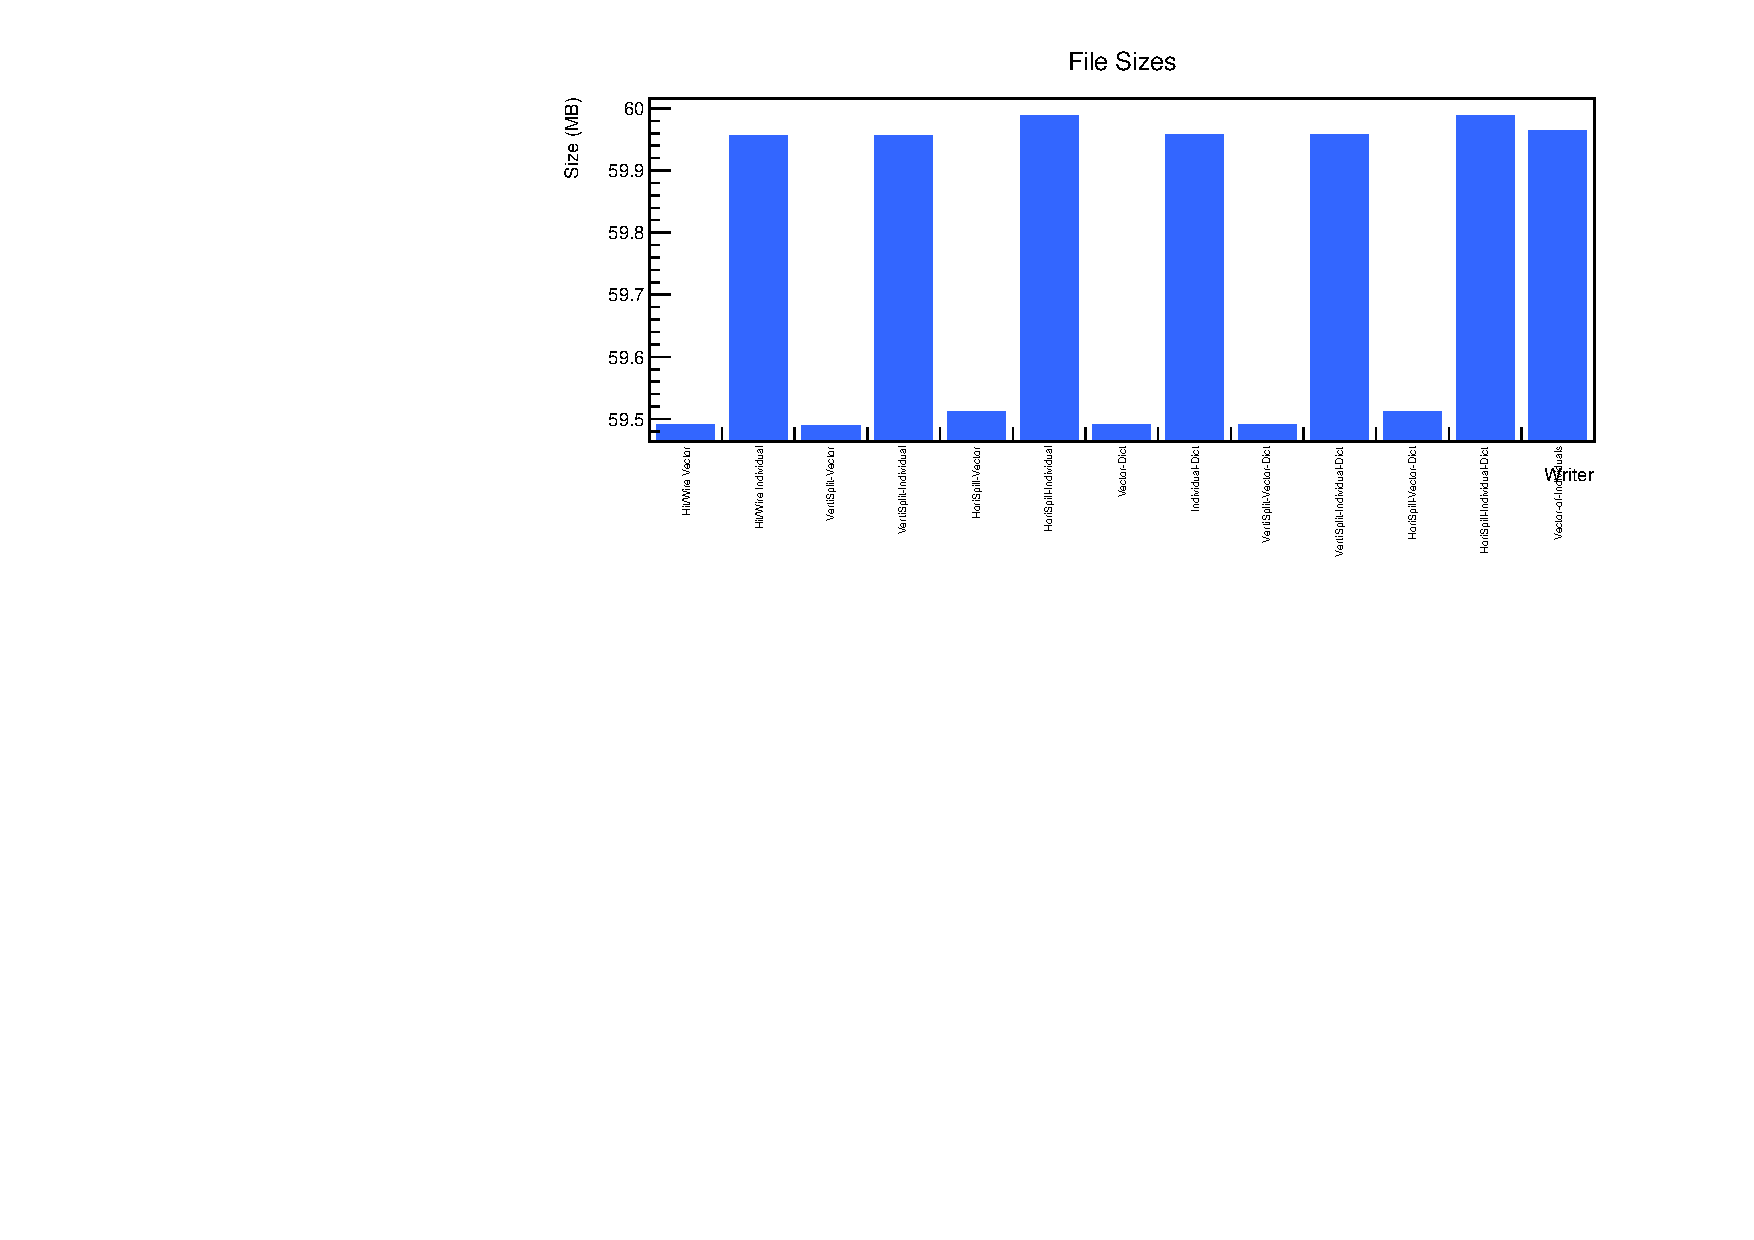
\includegraphics[width=0.9\linewidth]{../experiments/file_sizes.pdf}
\captionof{figure}{Experiment 2: Description goes here.}
\end{frame}

\begin{frame}{Experiment 3}
\centering
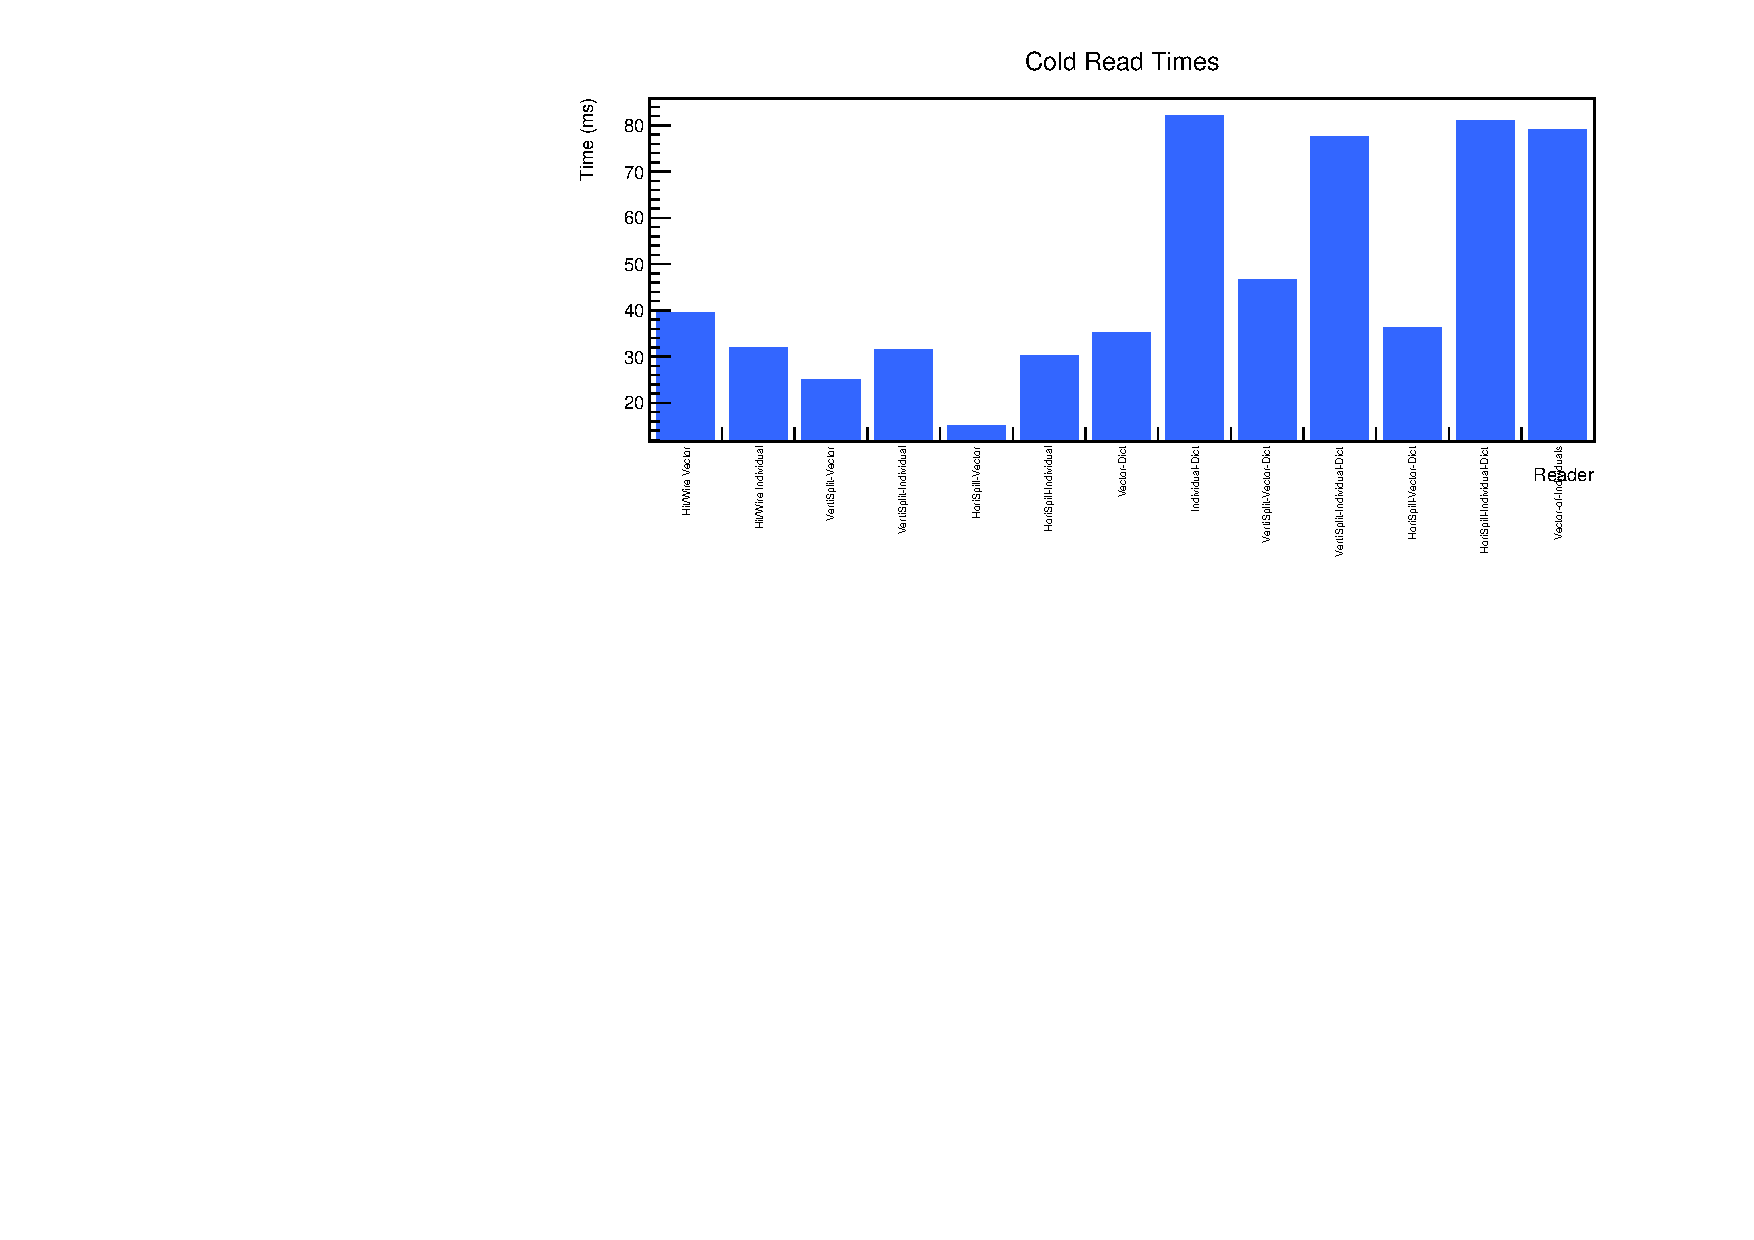
\includegraphics[width=0.9\linewidth]{../experiments/cold_times.pdf}
\captionof{figure}{Experiment 3: Description goes here.}
\end{frame}

\begin{frame}{Experiment 4}
\centering
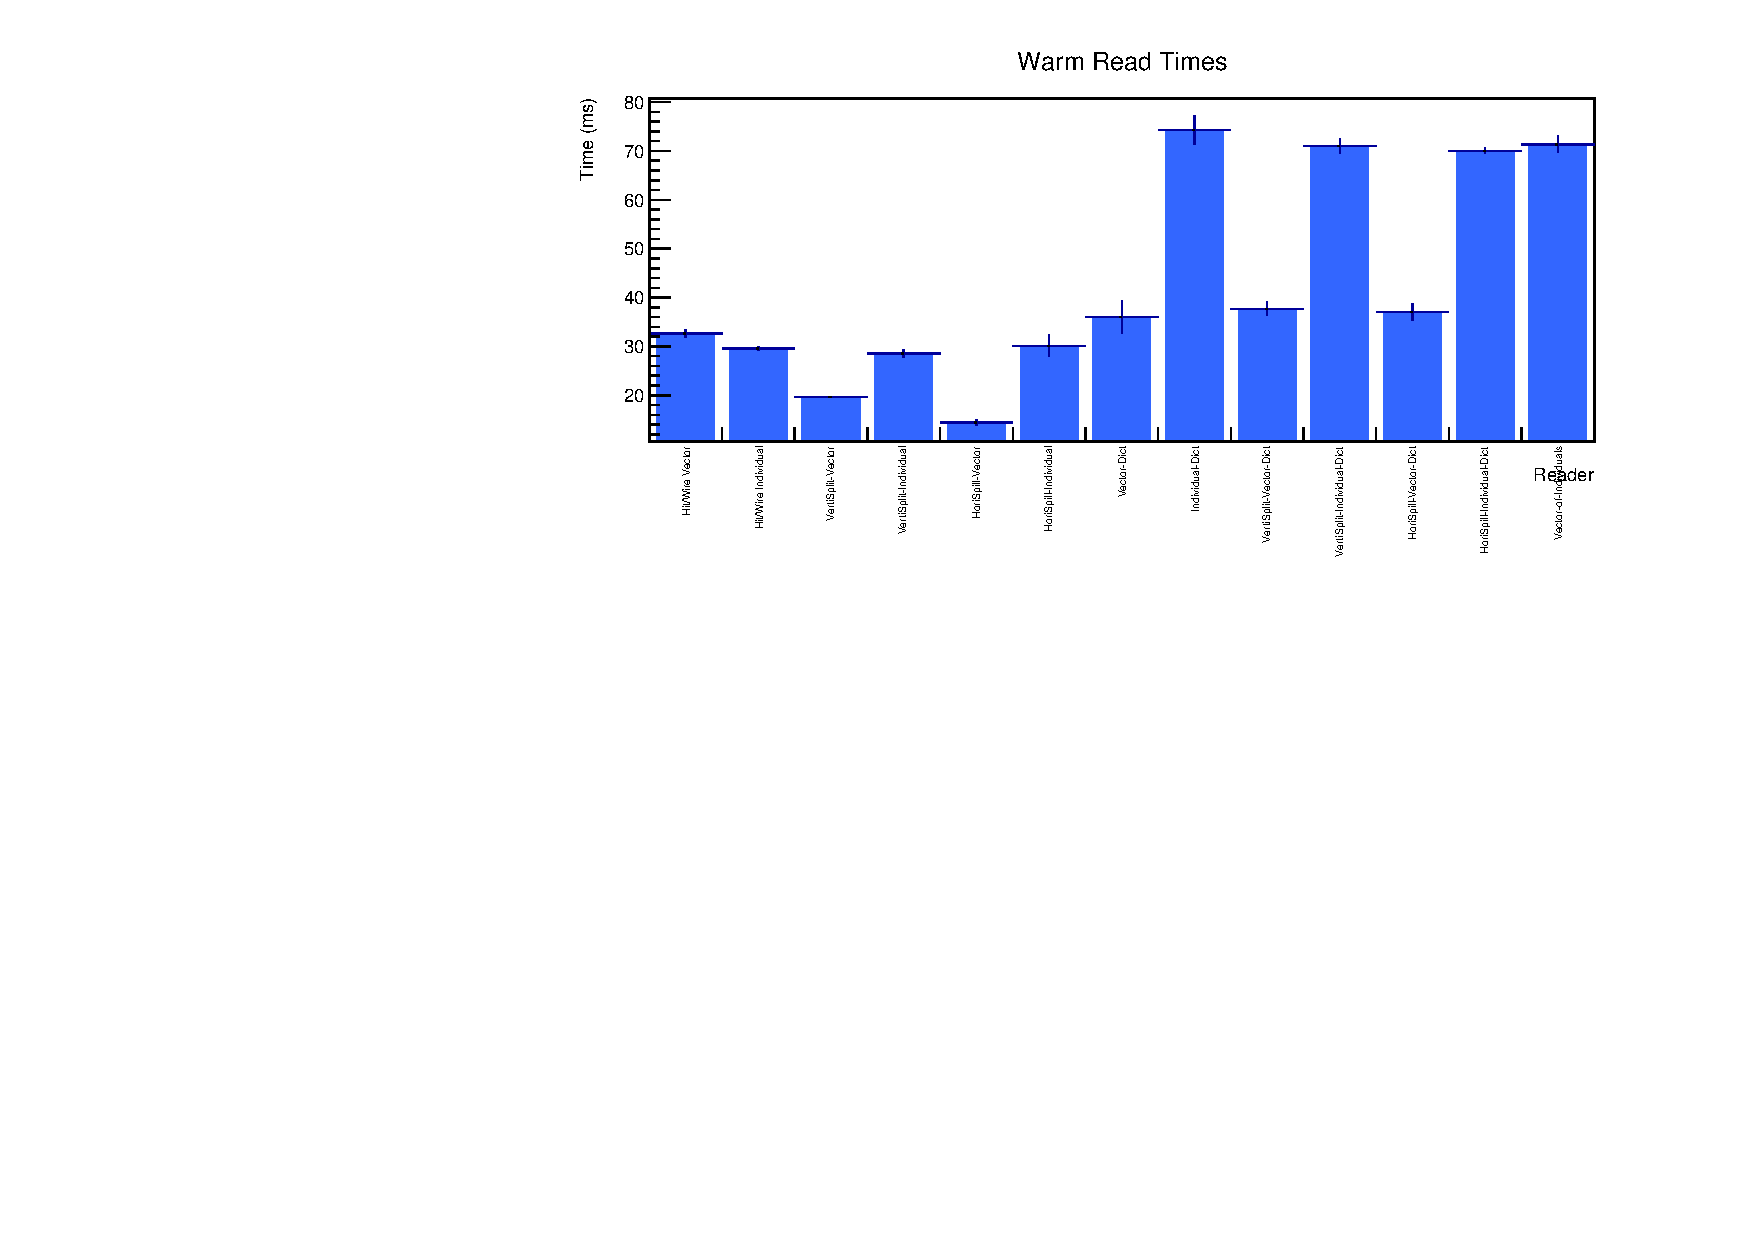
\includegraphics[width=0.9\linewidth]{../experiments/warm_times.pdf}
\captionof{figure}{Experiment 4: Description goes here.}
\end{frame}

\begin{frame}{Experiment 5}
\centering
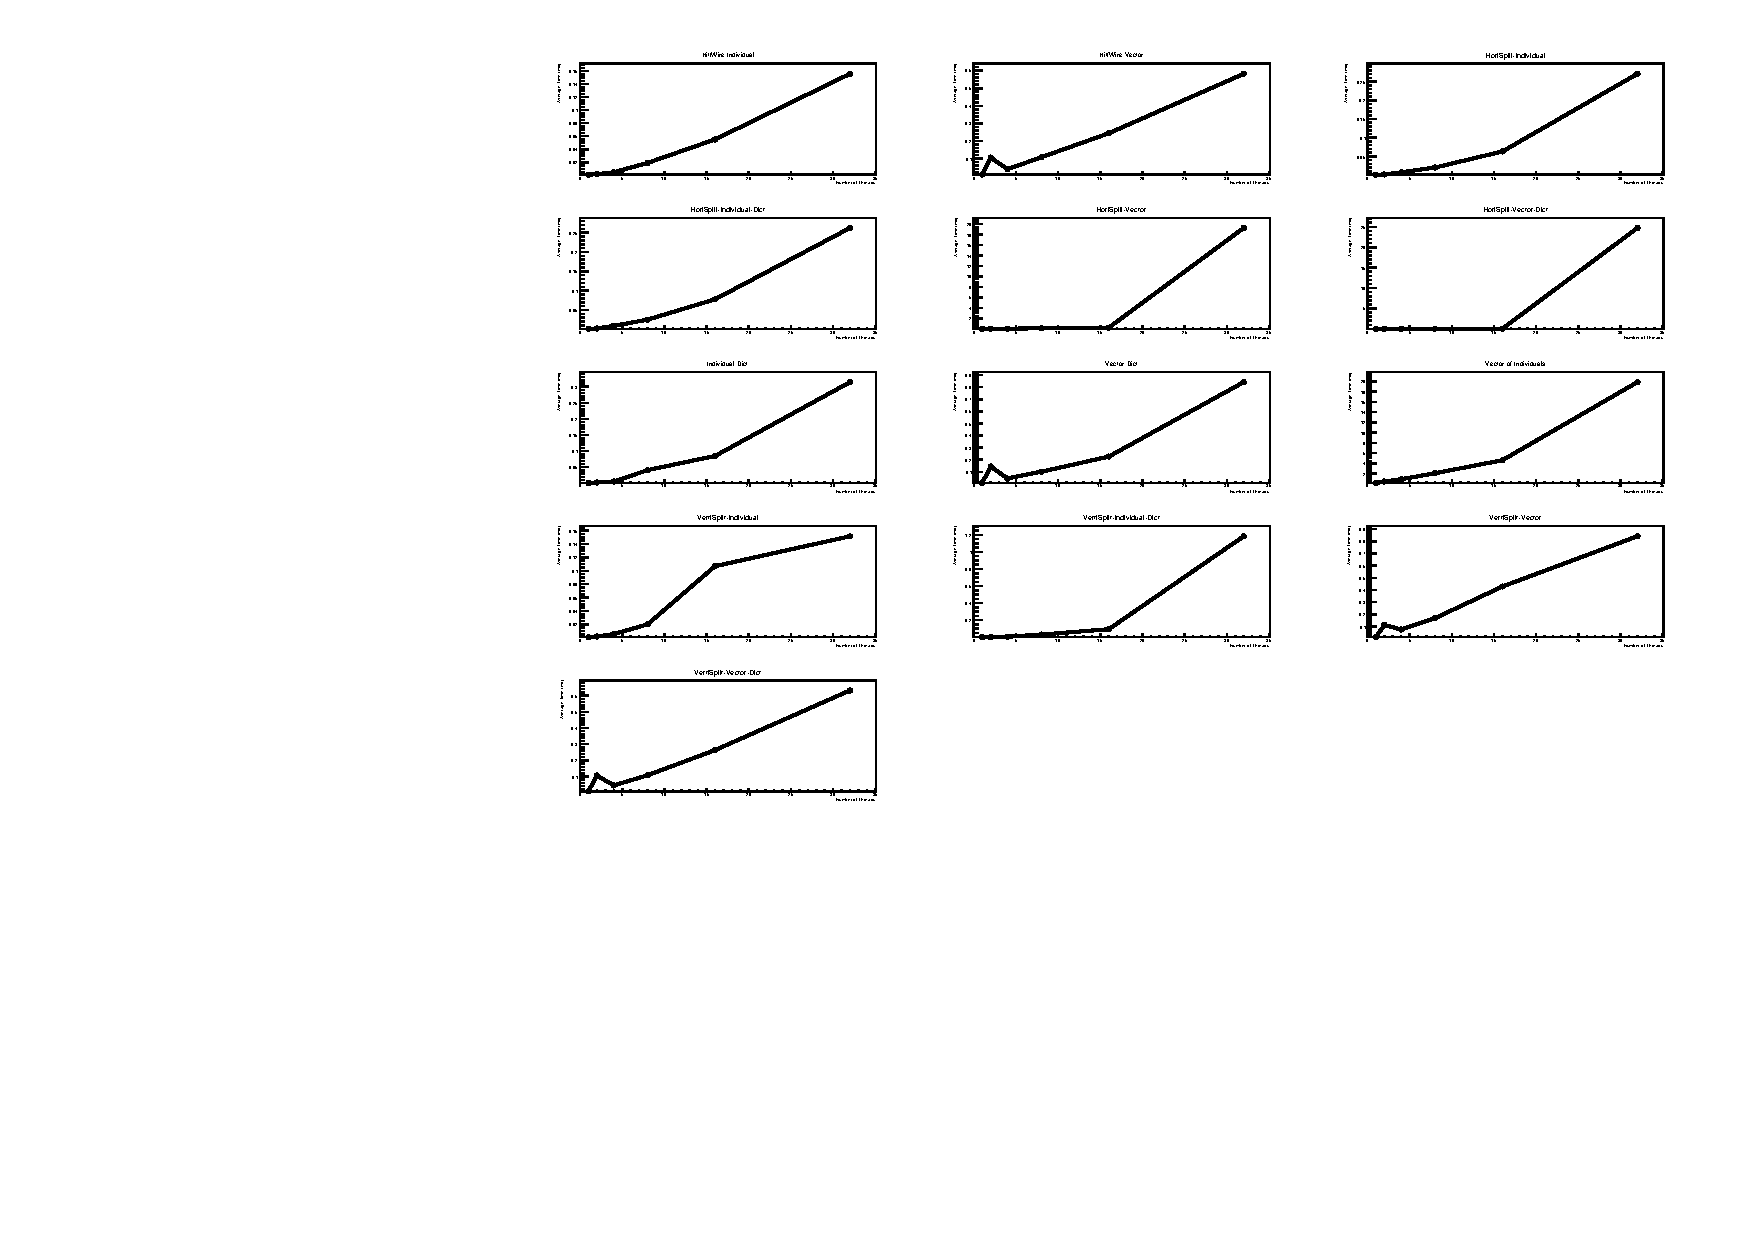
\includegraphics[width=0.9\linewidth]{../experiments/scaling_plot.pdf}
\captionof{figure}{Experiment 5: Description goes here.}
\end{frame}

% -------- Section: Trade-offs --------
\section{Trade-offs}
\begin{frame}{Design Trade-offs}
% Add your content here
\end{frame}

\begin{frame}{Future Considerations}
% Add your content here
\end{frame}

% Final Slide
\begin{frame}[standout]
Thank you! \\
Questions?
\end{frame}

\end{document}
